\newpage
\section{Factoren en Invloed}
\label{h5}



\subsection*{Deelvraag 2: Welke factoren kunnen per bevolkingsgroep van invloed zijn op het wel of niet behalen van het maximum aantal kandidaten dat in de Tweede Kamer gekozen kan worden?}
Voor het behalen van het maximum per bevolkingsgroep zijn er een aantal factoren die van invloed kunnen zijn. Deze factoren kunnen invloed uitoefenen op mate van een succes van een door een bevolkingsgroep gekozen strategie. Alvorens we per specifieke bevolkingsgroep de factoren en de invloed van deze factoren gaan beschrijven, zullen we eerst de algemene factoren beschrijven die van invloed (kunnen) zijn op elke bevolkingsgroep.

\subsubsection*{Algemene Factoren.}
De algemene factoren zijn de factoren die van invloed kunnen zijn op elke bevolkingsgroep. In deze sectie worden deze algemene factoren kort beschreven alvorens in de volgende secties er per specifieke bevolkingsgroep dieper op de factoren wordt ingegaan. De algemene factoren zijn:\\

\newcolumntype{L}{@{}>{\bfseries}p{14em}<{}}% Item label
\newcolumntype{I}{X@{}}% Item contents
\noindent\begin{tabularx}{\textwidth}{LI}
Aantal kandidaten: &  Voor het kunnen toepassen van één van de in het vorige hoofdstuk beschreven strategie\"{e}n, is het in eerste instantie essentieel dat er \"{u}berhaupt kandidaten van een bevolkingsgroep op de kandidatenlijsten staan. Daarnaast is het aantal kandidaten van belang om bijvoorbeeld een volledig door één bevolkingsgroep bezette Tweede Kamer te vormen. In de volgende secties betreffende de factoren per bevolkingsgroep wordt hier dieper op ingegaan. \\
\\ 
Keuze strategie: &  Een keuze van een strategie kan van invloed zijn op het wel of niet behalen van het theoretisch maximum. De keuze strategie voor een strategie kan complexiteit met zich meebrengen wat betreft de wijze van uitvoering.\\
\\ 
Committeren aan strategie:  & In het vorige hoofdstuk is telkens per bevolkingsgroep onderzocht wat het theoretisch maximum is wanneer 100\% van de kiesgerechtigden zich committeert aan een strategie. Echter is het de vraag wat er gebeurt als een bepaald percentage van een bevolkingsgroep zich committeert aan een strategie. Waar het theoretisch maximum uitgaat van 100\% deelname van de leden van een bevolkingsgroep is dit in de praktijk moeilijk haalbaar. Daarom zal er onderzocht worden het theoretisch maximum per bevolkingsgroep zou zijn geweest wanneer de meeste succesvolle strategie\"{e}n uit het vorige hoofdstuk zouden uitgevoerd door een deel van de bevolkingsgroep. Om een beeld te schetsen beperken we ons hierbij tot strategie 1 en strategie 2.  \\
\\
\end{tabularx}  
 
 \newcolumntype{L}{@{}>{\bfseries}p{14em}<{}}% Item label
\newcolumntype{I}{X@{}}% Item contents
\noindent\begin{tabularx}{\textwidth}{LI}

Tegenstrategie: & Een bevolkingsgroep met tegengestelde eigenschappen (bijvoorbeeld de bevolkingsgroep mannen tegenover vrouwen) of tegengestelde belangen zou een tegenstrategie  kunnen toepassen om te verhinderen dat de andere bevolkingsgroep(en) in hogere mate vertegenwoordigd worden in de Tweede Kamer. In Hoofdstuk \ref{h7} wordt er dieper ingegaan op wat er kan gebeuren wanneer meerdere bevolkingsgroepen een strategie uitvoeren.\\
\\
 \end{tabularx}  


\paragraph{Overzicht bevindingen.}
Voordat we per bevolkingsgroep dieper in gaan op de factoren en de invloed die deze factoren hebben, worden hieronder eerst de belangrijkste bevindingen op een rijtje gezet. De bevindingen zijn:

\begin{itemize}
\item
Wat betreft de Tweede Kamerverkiezingen van 2012, hadden alle bevolkingsgroepen een voldoende aantal kandidaten op de kandidatenlijsten staan. Enkel de SGP had zowel geen vrouwelijke alsmede allochtone kandidaten op de kandidatenlijst staan. De Partij voor de Dieren had geen allochtone kandidaten op de kandidatenlijst staan.
\item
Strategie 1 en strategie 2 zouden bij een deelname van slechts 40\% van de leden van de bevolkingsgroepen een hoog rendement hebben opgeleverd.
\item
De bevolkingsgroep vrouwen lijkt de bevolkingsgroep te zijn waar de meeste animo onder de bevolkingsleden bestaat als het gaat om het committeren aan een strategie om zodoende adequater vertegenwoordigd te worden in de Tweede Kamer. 
\item
Wat betreft het hanteren van een tegenstrategie is het moeilijk te concluderen welke bevolkingsgroepen het meest waarschijnlijk zouden kunnen worden tegengewerkt wanneer zij een strategie uit willen voeren. Echter lijkt het bij de bevolkingsgroep allochtonen en, in minder mate, de bevolkingsgroep vrouwen het meest waarschijnlijk dat er vanuit de samenleving een tegenbeweging kan ontstaan.
\end{itemize}



\subsection{Factoren Bevolkingsgroep Vrouwen.}
\label{percV}

\paragraph{Aantal vrouwelijke kandidaten.}
Zoals in het vorige hoofdstuk al is beschreven was het bij de Tweede Kamerverkiezingen van 2012 onmogelijk om een Tweede Kamer te vormen die volledig werd bezet door vrouwelijke kamerleden. De SGP had helemaal geen vrouwelijke kandidaten op de kandidatenlijst en de PVV en de VVD hadden een hoger aantal zetels ontvangen dan het aantal vrouwelijke kandidaten dat deze partijen op de kandidatenlijsten hadden. Echter waren er bij de partijen die zetels hebben ontvangen toch het totaal van 179 vrouwelijke kandidaten waarop gestemd kon worden(zie Figuur \ref{fig:aaKandidaten} in Hoofdstuk  \ref{sec:math}). 

\paragraph{Keuze strategie.}
Wat betreft het kiezen van een strategie is strategie 1 de strategie die bij de bevolkingsgroep vrouwen het meeste succes zou hebben opgeleverd. Zoals we weten, zou strategie 1 het maximum van 121 vrouwen in de Tweede Kamer op hebben kunnen leveren. Echter zou strategie 2 met 116 vrouwen in de Tweede Kamer ook een hoog rendement hebben opgeleverd. In de volgende paragraaf wordt er dieper ingegaan op wat er had gebeurd wanneer een deel van de bevolkingsgroep zich zou hebben gecommitteerd aan strategie 1 of strategie 2.

\paragraph{Committeren aan een strategie.}
Sinds de dagen van Aletta Jacobs en het ontstaan van de \textit{Eerste Feministische Golf} \citep{braun1992prijs}, de \textit{Dolle Mina's} en de \textit{Man Vrouw Maatschappij} in de jaren '60 en het ontstaan van de \textit{Tweede Feministische Golf} \citep{van2005vrouw} zijn er in de loop der jaren tal van personen en organisaties in Nederland bij gekomen die de belangen van vrouwen behartigen. Een kleine greep uit Nederlandse vrouwenbelangen organisaties levert op: de Nederlandse Bond voor Vrouwenkiesrecht, Nederlandse Unie voor Vrouwenbelangen, de Nederlandse Vrouwenraad, FNV Vrouw, Vereniging Vrouw en Recht etc. Daarnaast is minister Bussemaker van Onderwijs, Cultuur en Wetenschap \citeyearpar{navigerennaardetop} campagne begonnen die ervoor moet zorgen dat er meer vrouwen in topfuncties komen in Nederland. Volgens \cite{van2012tweede} ontvangen met name de hoogstgeplaatste vrouwelijke kandidaten op de kandidatenlijsten een voorkeurstem van de vrouwelijke kiezer vanwege het feit dat de kandidaat van hetzelfde geslacht is. Tevens is het zo dat bij de Tweede Kamerverkiezingen van 2012 \citep{Kiesraad_uitslag} de hoogstgeplaatste vrouwelijke kandidaten op de kandidatenlijsten (de vrouwelijke lijsttrekkers buiten beschouwing gelaten) een hoog aantal voorkeurstemmen ontvingen. In Tabel \ref{table:HoogstV} is te zien dat zeven hoogstgeplaatste vrouwelijke kandidaten genoeg stemmen hadden ontvangen om boven de voorkeursdrempel uit te komen. Het gemiddelde bij de hoogstgeplaatste vrouwelijke kandidaten lag maar liefst op het aantal van 66.419 stemmen. Er kan worden aangenomen dat er een zekere animo bestaat bij Nederlandse vrouwen om zich te committeren aan een strategie die ervoor moet zorgen dat vrouwen in hogere mate vertegenwoordigd worden in de Tweede Kamer. 


\begin{table}[H]
\centering
	\begin{footnotesize}
		\begin{tabular}{llrr}
\toprule
{} &                 Partij &  Plaats op Lijst &  Aantal Stemmen  \\
Kandidaat                                &                        &                  &    Kandidaat                       \\
\midrule
M.H.H. (Martine) Baay-Timmerman          &                 50PLUS &                3 &                      7123 \\
M.C.G. (Mona) Keijzer                    &                    CDA &                2 &                    127446 \\
C.J. (Carola) Schouten                   &           ChristenUnie &                3 &                     16507 \\
S. (Stientje) van Veldhoven-van der Meer &                    D66 &                2 &                     71170 \\
L. (Liesbeth) van Tongeren               &             GROENLINKS &                3 &                     10205 \\
E. (Esther) Ouwehand                     &  Partij v d Dieren &                2 &                     11573 \\
J. (Jetta) Klijnsma                      &                   PVDA &                2 &                    192190 \\
M. (Fleur) Agema                         &                    PVV &                2 &                     34943 \\
R.M. (Renske) Leijten                    &                     SP &                2 &                     69146 \\
E.I. (Edith) Schippers                   &                    VVD &                2 &                    123889 \\
\bottomrule
\end{tabular}

	\end{footnotesize}
			\caption{Het aantal stemmen dat de hoogstgeplaatste vrouwelijke kandidaten hebben ontvangen volgens de offci\"{e}le einduitslag \citep{Kiesraad_uitslag}. De SGP had geen vrouwelijke kandidaten.}
\label{table:HoogstV} 
\end{table} 

Een deelname van 100\% van de vrouwelijke kiezers aan strategie 1 zou een Tweede Kamer op hebben kunnen leveren waarin 121 vrouwen plaats zouden hebben genomen en bij strategie 2 zouden er 116 vrouwen plaats hebben genomen (zie Sectie \ref{vrouwen}. Echter is het de vraag wat er had gebeurd wanneer niet de volle 100\% van de vrouwelijke kiezers zich had gecommitteerd maar een 'slechts' een deel van de vrouwelijke kiezers. In Figuur \ref{fig:PerV} is te zien hoeveel zetels er aan vrouwelijk kandidaten bedeeld zouden zijn wanneer een bepaald percentage van de vrouwelijke kiezers zich had gecommitteerd aan strategie 1 (blauwe staven) of strategie 2 (groene staven). Hierbij moet genoteerd worden dat het aantal stemmen van vrouwelijke kiezers op een partij een percentage is van het totaal door vrouwelijke kiezers uitgebrachte stemmen. Tevens nemen we aan dat het percentage van de vrouwelijke kiezers die zich committeren aan een strategie voor elke partij hetzelfde is. Oftewel wanneer bijvoorbeeld 25\% van de vrouwelijke kiezers zich committeren aan de strategie dan is geldt de 25\% voor elke partij. Ter illustratie het nemen we de VVD als voorbeeld.

De VVD had volgens de einduitslag van de Tweede Kamerverkiezingen van 2012 een totaal van 1.077.127 vrouwelijke stemmen ontvangen (zie Figuur \ref{table:tab2V} in Sectie \ref{vrouwen}). Wanneer 25\% van de vrouwelijke kiezers zich hadden gecommitteerd aan strategie 1 of strategie 2 zouden deze strategie\"{e}n bij de VVD het aantal van ($25\%*1.077.127$ = ) 269.281 vrouwelijke stemmen hebben opgeleverd ten behoeve aan de strategie. De overige stemmen van vrouwelijke kiezers op de VVD laten we buiten beschouwing vanwege het feit dat we niet kunnen voorspellen naar welke partij of kandidaat deze stemmen gegaan zouden zijn. Derhalve kunnen we alleen het aantal stemmen in ogenschouw nemen wat zekerheid biedt voor het berekenen van het aantal stemmen dat vrouwelijke kandidaten van vrouwelijk kiezers zouden gaan ontvangen om zodoende vrouwelijke kandidaten aan de kiesdrempel te helpen.  

In Figuur \ref{fig:PerV} is te zien dat wanneer slechts 70\% van de vrouwelijke kiezers zich had gecommitteerd aan strategie 1, het maximum aantal nog altijd zou zijn behaald. Bij 60\% van de vrouwelijke kiezers viel er bij strategie 1 één enkele vrouwelijke kandidaat af en bij slechts 50\% van de vrouwelijke kiezers zouden er nog altijd 36 vrouwen meer in de Tweede Kamer plaats hebben genomen dan daadwerkelijk bij de offci\"{e}le einduitslag het geval was (58 vrouwen in de Tweede Kamer na de offci\"{e}le einduitslag). Voor strategie 2 is te zien dat het maximum aantal dat mogelijk zou zijn geweest met uitvoering van strategie 2, behaald zou zijn geweest wanneer 85\% van de vrouwelijke kiezers zich had gecommitteerd aan strategie 2. Bij slechts 50\% van de vrouwelijke kiezers zouden er nog altijd 33 vrouwen meer in de Tweede Kamer plaats hebben genomen dan daadwerkelijk bij de offci\"{e}le einduitslag het geval was.

\begin{figure}[H]


	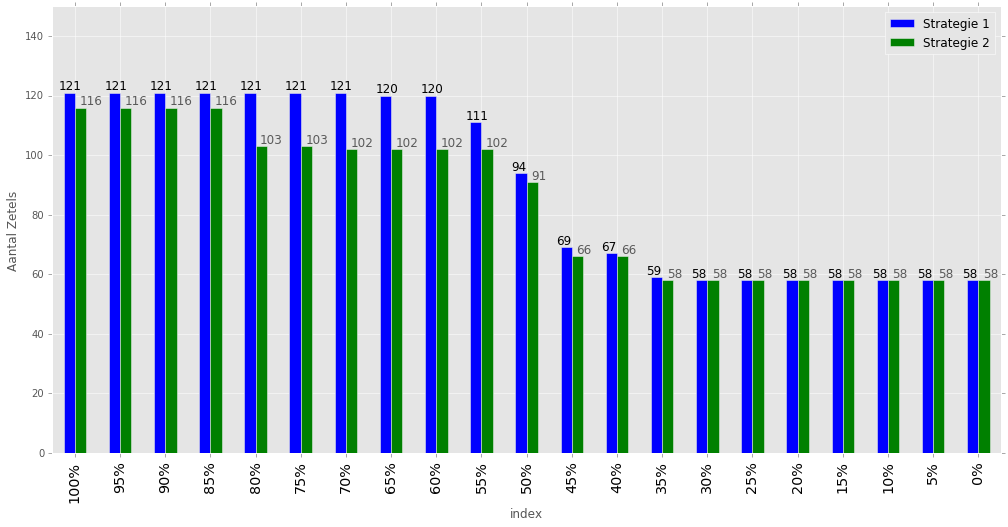
\includegraphics[width=\linewidth]{percentages_van_vrouwenS1S2.png}

			\caption{Grafiek met overzicht van het maximum aantal zetels wat behaald kon worden wanneer een bepaald percentage van de vrouwelijke kiezers zich committeerde aan strategie 1 of strategie 2.}

\label{fig:PerV}
\end{figure}






\paragraph{Tegenstrategie.}
Uit een onderzoek van \cite{lawless2012men} blijkt dat mannen in de Verenigde Staten het eigen geslacht geschikter achten voor het bekleden van een politieke ambt dan het vrouwelijk geslacht. Een vergelijkbaar onderzoek betreffende mannen en vrouwen in Nederland ontbreekt echter. Hoewel een onderzoek van \cite{mcelroy2009candidate} aangeeft dat kiezers in landen waar verkiezingen met een voorkeursstemregel niet discrimineren op basis van geslacht, is het mogelijk dat mannen het eigen geslacht prefereren als het gaat om het kiezen van vertegenwoordigers in de Tweede Kamer. Zodoende is het niet ondenkbaar dat mannen een tegenstrategie zullen toepassen om te voorkomen dat de vrouwen in hogere mate vertegenwoordigd worden dan ooit het geval is geweest. 

\subsection{Factoren Bevolkingsgroep Allochtonen.}

\paragraph{Aantal allochtone kandidaten.} 
Zoals in het vorige hoofdstuk al is beschreven was het bij de Tweede Kamerverkiezingen van 2012 onmogelijk om een Tweede Kamer te vormen die volledig werd bezet door allochtone politici. De SGP en de Partij voor de Dieren hadden geen enkele allochtoon op de kandidatenlijsten staan en, op 50PLUS en GROENLINKS na, ontvingen alle partijen bij de einduitslag meer zetels dan het aantal allochtonen dat zij op de kandidatenlijsten hadden staan. In totaal stonden er, bij de partijen die zetels hebben ontvangen, vijftig allochtone kandidaten op de kandidatenlijsten (zie Figuur \ref{fig:aaKandidaten} in Hoofdstuk \ref{sec:meth}). 

\paragraph{Keuze strategie.}
Wat betreft het kiezen van een strategie maakt het voor de bevolkingsgroep allochtonen niet uit of strategie 1 of strategie 2 wordt uitgevoerd wanneer de volle 100\% van de allochtone kiezers zich committeren aan de strategie. Ook bij het uitvoeren van strategie 2 waarbij slechts een deel van de allochtone kiezers zich committeert aan de strategie is het resultaat hetzelfde. Het maakt geen verschil of er voor strategie 1 of strategie 2 wordt gekozen. In de volgende paragraaf wordt er dieper ingegaan op wat er had gebeurd zou zijn wanneer een deel van de bevolkingsgroep zich zou hebben gecommitteerd aan strategie 1 of strategie 2.



\paragraph{Committeren aan een strategie.}
Uit onderzoek van \cite{fennema2001civic} blijkt dat met name allochtonen van Turkse en Marokkaanse afkomst geneigd zijn op een kandidaat te stemmen met dezelfde afkomst. Echter lijken allochtone kiezers van Turkse afkomst in hogere mate te mobiliseren als het gaat om het uitbrengen van een stem bij de Tweede Kamerverkiezingen dan allochtonen van Marokkaanse afkomst. Onderzoek betreffende allochtonen met een andere afkomst dan een Turkse of Marokkaanse ontbreekt echter. Als het gaat om verbondenheid tussen etnische minderheden voelen personen behorende tot verschillende etnische minderheden zich in sterkere mate met elkaar verbonden wanneer zij zich benadeeld of minder geaccepteerd voelen \citep{schmitt2002meaning}. Volgens \cite{buijs2006strijders} voelen veel allochtonen in Nederland, van met name Turkse en Marokkaanse achtergrond, zich niet geaccepteerd. Volgens \cite{van2012tweede} geldt ook voor allochtonen dat zij in de meeste voorkeurstemmen uitbrengen op de hoogstgeplaatste allochtone kandidaat op de kandidatenlijst. In Tabel \ref{table:HoogstA} is te zien dat van de hoogstgeplaatste allochtone kandidaten op de kandidatenlijsten er slechts één allochtone kandidaat, in de persoon van Tanja Jadnanansing, boven de voorkeursdrempel uit is gekomen. Of dit ligt aan het feit dat zij stemmen van allochtone kiezers heeft gekregen, stemmen van vrouwelijke kiezers heeft gekregen of een combinatie van beiden is niet duidelijk. Het gemiddelde bij de hoogstgeplaatste allochtone kandidaten lag op het aantal van 7.420 stemmen. Afgaande op het het aantal stemmen op de hoogstgeplaatste allochtone kandidaat lijkt de stelling van \cite{van2012tweede} niet helemaal op te gaan. Echter kan uit de eerdere stelling in deze paragraaf wel worden afgeleid dat er animo kan bestaan onder allochtonen om zich te committeren aan een strategie die ervoor moet zorgen dat allochtonen in hogere mate vertegenwoordigd worden in de Tweede Kamer. \\

\begin{table}[H]
\centering
	\begin{footnotesize}
		\begin{tabular}{lllrr}
\toprule
{} & Geslacht &        Partij &  Plaats op Lijst &  Aantal Stemmen Kandidaat \\
Kandidaat                 &          &               &                  &                           \\
\midrule
K.L.R. (Roy) Ho Ten Soeng &        M &        50PLUS &                6 &                      2654 \\
M. (Mustafa) Amhaouch     &        M &           CDA &               16 &                      1919 \\
I.S. (Ixora) Balootje     &        V &  ChristenUnie &                9 &                      2111 \\
V.A. (Vera) Bergkamp      &        V &           D66 &                5 &                     15387 \\
J.F. (Jesse) Klaver       &        M &    GROENLINKS &                4 &                      3351 \\
T.M. (Tanja) Jadnanansing &        V &          PVDA &                4 &                     28704 \\
J.D. (Jenny) Zerfowski    &        V &           PVV &               37 &                       210 \\
S. (Sadet) Karabulut      &        V &            SP &                6 &                     10572 \\
M. (Malik) Azmani         &        M &           VVD &               20 &                      1874 \\
\bottomrule
\end{tabular}

	\end{footnotesize}
			\caption{Het aantal stemmen dat de hoogstgeplaatste allochtone kandidaten hebben ontvangen volgens de offci\"{e}le einduitslag \citep{Kiesraad_uitslag}.}
\label{table:HoogstA} 
\end{table}





\indent Een deelname van 100\% van de allochtone kiezers aan strategie 1 of strategie 2 zou een Tweede Kamer hebben opgeleverd waarin 34 allochtonen plaatsen zouden nemen (zie Sectie \ref{allochtonen}). Ook bij de bevolkingsgroep allochtonen gaan we onderzoek wat er zou zijn gebeurd wanneer een deel van de bevolkingsgroep zich committeert aan strategie 1 of strategie 2. Op dezelfde wijze als bij de bevolkingsgroep vrouwen is gedaan, gaan we berekenen hoeveel zetels er aan allochtone kandidaten bedeeld zouden zijn wanneer bepaalde percentages van de bevolkingsgroep allochtonen zich had gecommitteerd aan strategie 1 of strategie 2 (zie Sectie \ref{percV} voor uitleg van het berekenen van het aantal stemmen). In Figuur\ref{fig:PerA} is te zien hoeveel zetels er aan allochtone kandidaten zouden zijn bedeeld wanneer een bepaald percentage van de allochtone kiezers zich had gecommitteerd aan strategie 1 (blauwe staven) of strategie 2 (groene staven).  

\begin{figure}[H]


	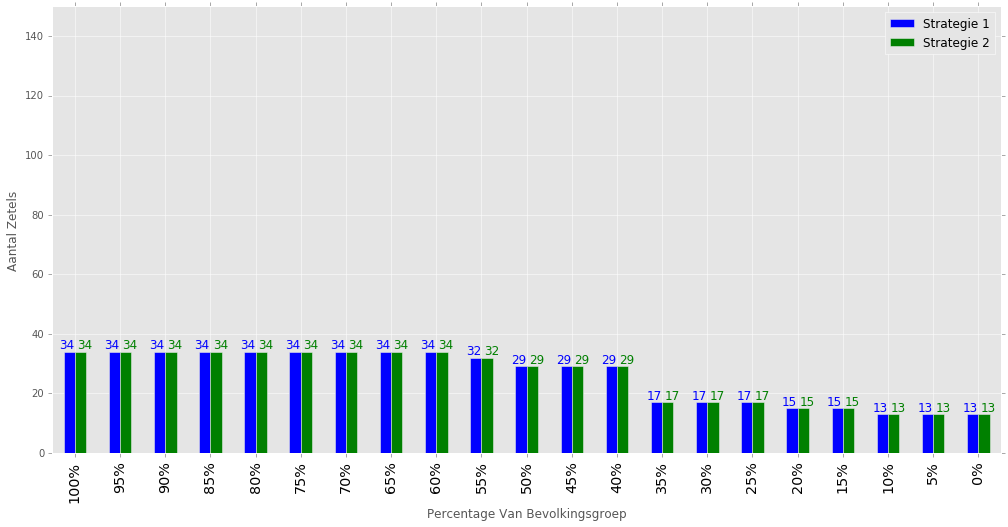
\includegraphics[width=\linewidth]{percentages_van_allochtonenS1S2.png}

			\caption{Grafiek met overzicht van het maximum aantal zetels wat behaald kon worden wanneer een bepaald percentage van de allochtone kiezers zich committeerde aan strategie 1 of strategie 2.}

\label{fig:PerA}
\end{figure}

In Figuur \ref{fig:PerA} is te zien dat wanneer slechts 60\% van de allochtone kiezers zich had gecommitteerd aan strategie 1 of strategie 2, het maximum aantal nog altijd werd behaald. Bij 40\% van de allochtone kiezers zouden er vijf allochtone kandidaten afgevallen zijn en bij slechts 25\% van de allochtone kiezers zouden er bij beiden strategie\"{e}n nog altijd vier allochtonen meer in de Tweede Kamer terecht gekomen zijn dan daadwerkelijk bij de offci\"{e}le einduitslag het geval was (dertien allochtonen in de Tweede Kamer na de offci\"{e}le einduitslag). Beiden strategie\"{e}n hadden voor elk percentage aan deelnemers hetzelfde rendement opgeleverd.




\paragraph{Tegenstrategie.}
Volgens een artikel van \cite{de2000political} blijkt het zo te zijn dat rechtse partijen in zowel Nederland als Vlaanderen (bijvoorbeeld het Vlaams Blok) kiezers voor zich weten te winnen op basis van een negatief beeld dat deze kiezers hebben als het gaat om allochtonen- en migrantenkwesties. Daarnaast speelt ook chauvinisme een rol als het gaat om het stemmen op autochtone kandidaten en populistische partijen \citep{van2010swaying}. Hierdoor is het niet ondenkbaar dat een groep autochtone kiezers een tegenstrategie zal uitvoeren om juist meer autochtone kandidaten in de Tweede Kamer te krijgen.

\subsection{Factoren Bevolkingsgroep Ouderen.}
\label{percO}

\paragraph{Aantal oudere kandidaten.} 
Zoals in het vorige hoofdstuk al is beschreven was het bij de Tweede Kamerverkiezingen van 2012 onmogelijk om een Tweede Kamer te vormen die volledig werd bezet door oudere politici. Het CDA, de PVDA, de VVD, de SP, D66 en de SGP ontvingen meer zetels dan dat zij oudere kandidaten op de kandidatenlijst hadden staan. In totaal stonden er, bij de partijen die zetels hebben ontvangen, 135 oudere kandidaten op de kandidatenlijsten (zie Figuur \ref{fig:jaKandidaten} in Hoofdstuk \ref{sec:math})

\paragraph{Keuze strategie.}
Wat betreft het kiezen van een strategie is strategie 1 de strategie die bij de Tweede Kamerverkiezingen van 2012 het meeste rendement zou hebben opgeleverd bij de bevolkingsgroep ouderen. Strategie 1 zou het maximum van 89 ouderen in de Tweede Kamer hebben opgeleverd. Echter zou strategie 2 met 84 ouderen in de Tweede Kamer ook een hoog rendement hebben opgeleverd. In de volgende paragraaf wordt er dieper ingegaan op wat er had gebeurd wanneer een deel van de bevolkingsgroep zich zou hebben gecommitteerd aan strategie 1 of strategie 2.

\paragraph{Committeren aan een strategie.}
In de literatuur bestaat er geen onderzoek betreffende voorkeurstemmen op oudere kandidaten. Echter kan aan de hand van de verkiezingseinduitslag worden opgemaakt dat er weinig sentimenten leven onder ouderen om beter vertegenwoordigd te worden door oudere politici in de Tweede Kamer. Een partij die specifiek opkomt voor belangen van ouderen is 50PLUS. Het feit dat 50PLUS slechts 4\% van de stemmen van ouderen heeft gekregen (zie Figuur \ref{fig:zetelsO} in Sectie \ref{ouderen}) suggereert dat ouderen ook andere aandachtspunten dan het zijn van een oudere belangrijk vinden als het gaat om het uitbrengen van een stem. Tevens is het zo dat de hoogstgeplaatste ouderen op de kandidatenlijsten (de lijsttrekkers buiten beschouwing gelaten) over het algemeen weinig voorkeurstemmen hebben ontvangen. In Tabel \ref{table:HoogstO} is te zien dat enkel Fred Teeven van de VVD en Jetta Klijnsma van de PVDA genoeg stemmen hebben ontvangen om boven de voorkeursdrempel uit te komen. Echter genieten deze politici een grote mate van bekendheid in Nederland en stonden zij hoog op de kandidatenlijsten. Hetgeen een goeie indicatie is voor het krijgen van voorkeurstemmen \citep{van2012tweede}. Het gemiddelde bij de hoogstgeplaatste oudere kandidaten lag op het aantal van 22.937 stemmen. Echter wordt het gemiddelde door het grote aantal voorkeurstemmen dat Jette Klijnsma ontving flink omhoog gekrikt. Het feit dat Jetta Klijnsma zo veel stemmen heeft ontvangen ligt waarschijnlijk ten grondslag aan het feit dat, zoals eerder al is aangegeven, vrouwelijke kiezers geneigd zijn om op de hoogstgeplaatste vrouwelijke kandidaat te stemmen. Het lijkt daarmee onwaarschijnlijk dat Jetta Klijnsma zo veel stemmen heeft ontvangen vanwege het feit dat zij een oudere is. Dit alles doet vermoeden dat het onwaarschijnlijk lijkt dat ouderen zich zullen committeren aan een strategie. Desalniettemin, of misschien wel des te meer, is het interessant om te onderzoek wat het theoretisch maximum is wanneer een deel van de oudere kandidaten zich committeert aan een strategie. \\

\begin{table}[H]
\centering
	\begin{footnotesize}
		\begin{tabular}{lllrr}
\toprule
{} & Geslacht &                 Partij &  Plaats   &  Aantal Stemmen  \\
 & & & op Lijst & Kandidaat\\
Kandidaat                                &          &                        &                  &                           \\
\midrule
N.P.M. (Norbert) Klein       &        M &                 50PLUS &                2 &                      3511 \\
P. (Peter) Oskam             &        M &                    CDA &               10 &                       702 \\
C.P. (Onno) van Schayck      &        M &           ChristenUnie &               17 &                       307 \\
P.H. (Paul) van Meenen       &        M &                    D66 &                7 &                      1802 \\
A. (Bram) van Ojik           &        M &             GROENLINKS &                2 &                      4639 \\
B.E.J.M. (Birgit) Verstappen &        V &  Partij voor de Dieren &                7 &                       844 \\
J. (Jetta) Klijnsma          &        V &                   PVDA &                2 &                    192190 \\
L. (Louis) Bontes            &        M &                    PVV &                5 &                       958 \\
R. (Roelof) Bisschop         &        M &                    SGP &                3 &                      2234 \\
H. (Harry) van Bommel        &        M &                     SP &                4 &                     10021 \\
F. (Fred) Teeven             &        M &                    VVD &                5 &                     35103 \\
\bottomrule
\end{tabular}

	\end{footnotesize}
			\caption{Het aantal stemmen dat de hoogstgeplaatste oudere kandidaten hebben ontvangen volgens de offci\"{e}le einduitslag \citep{Kiesraad_uitslag}.}
\label{table:HoogstO} 
\end{table}

\newpage

\indent Een deelname van 100\% van de oudere kiezers aan strategie 1 zou in een Tweede Kamer hebben opgeleverd waarin 89 ouderen plaats zouden nemen en bij strategie 2 zouden er 84 ouderen hebben plaatsgenomen (zie Sectie \ref{ouderen}. Op dezelfde wijze als bij de bevolkingsgroep vrouwen is gedaan, gaan we berekenen hoeveel zetels er aan oudere kandidaten worden bedeeld wanneer bepaalde percentages van de bevolkingsgroep ouderen zich committeert aan de strategie (zie Sectie \ref{percV} voor uitleg van het bereken van het aantal stemmen). In Figuur \ref{fig:PerO} is te zien hoeveel zetels er aan oudere kandidaten zouden zijn bedeeld wanneer een bepaald percentage van de oudere kiezers zich had gecommitteerd aan strategie 1 of strategie 2.  



\begin{figure}[H]
	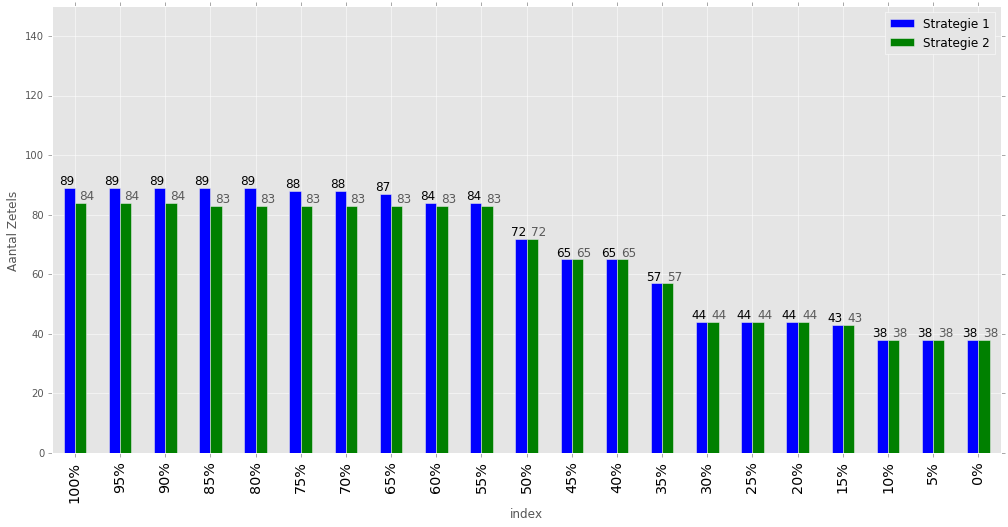
\includegraphics[width=\linewidth]{percentages_van_ouderenS1S2.png}

			\caption{Grafiek met overzicht van het maximum aantal zetels wat behaald kon worden wanneer een bepaald percentage van de oudere kiezers zich committeerde aan strategie 1 of strategie 2.}

\label{fig:PerO}
\end{figure}

In Figuur \ref{fig:PerO} is te zien dat wanneer 80\% van de oudere kiezers zich had gecommitteerd aan strategie 1, het maximum aantal nog altijd zou zijn behaald. Bij 55\% van de oudere kiezers vielen er vijf oudere kandidaten af en bij slechts 35\% van de oudere kiezers zijn er nog altijd negentien ouderen meer in de Tweede Kamer dan daadwerkelijk bij de offci\"{e}le einduitslag het geval was (38 ouderen in de Tweede Kamer na de offci\"{e}le einduitslag). Voor strategie 2 is te zien dat het maximum aantal dat mogelijk zou zijn geweest met uitvoering van strategie 2, behaald werd wanneer 90\% van de oudere kiezers zich had gecommitteerd aan strategie 2. Bij slechts 50\% van de oudere kiezers zouden er nog altijd 35 ouderen meer in de Tweede Kamer plaats hebben genomen dan daadwerkelijk bij de offci\"{e}le einduitslag het geval was. Bij 40\% van de oudere kiezers zouden er 27 ouderen meer in de Tweede Kamer hebben plaatsgenomen dan in 2012 het geval was.



\paragraph{Tegenstrategie.}
Volgens \cite{aalberts2006aantrekkelijke} vinden met name jongeren dat politici te oud zijn. Echter is het de vraag in hoeverre dit invloed zou kunnen hebben op hun partij- of kandidatenkeuze. Hoewel misschien onwaarschijnlijk, is het niet ondenkbaar dat een groep opstaat en zich samen aan een strategie committeert om zodoende te zorgen dat er juist minder oudere kandidaten in de Tweede Kamer plaatsnemen. 

\subsection{Factoren bevolkingsgroep provincialen.}
\label{percP}

\paragraph{Aantal Provinciale Kandidaten.} 
Bij \hyperref[S1A]{strategie 1} voor de bevolkingsgroep provincialen (zie Bijlage \ref{provincialen}) werd beschreven dat gezien de peiling en het bepalen van de top \textit{N} provinciale kandidaten er niet meer dan 147 provinciale kandidaten gekozen konden worden. Dit vanwege het feit dat de SP minder provinciale kandidaten op de kandidatenlijst had staan dan verwacht werd dat zij zetels zouden gaan ontvangen (zie Strategie \ref{sssec:S1P} in Sectie \ref{provincialen}). Echter de peiling correspondeerde niet 100\% met de uiteindelijke einduitslag. Op de PVDA na hadden alle partijen en hoger aantal provinciale kandidaten dan het aantal zetels dat zij a.d.h.v. de einduitslag bedeeld kregen. De PVDA had echter één zetels minder ontvangen dan het aantal provinciale kandidaten dat zij op de kandidatenlijsten hadden staan. Er hadden een totaal van 149 provincialen in de Tweede Kamer gekozen kunnen worden. Hierdoor had een Tweede Kamer bestaande uit enkel provincialen net niet mogelijk geweest. In totaal stonden er, bij de partijen die zetels hebben ontvangen, 235 oudere kandidaten op de kandidatenlijsten (zie Figuur \ref{fig:rpKandidaten} in Hoofdstuk \ref{sec:meth}).

\paragraph{Keuze strategie.}
Wat betreft het kiezen van een strategie is strategie 1 niet de strategie die het meeste succes opleverde bij de bevolkingsgroep provincialen. Zoals aangetoond bij de uitvoering van \hyperref[S4P]{strategie 4} in Bijlage \ref{provincialen}, leverde strategie 4 het theoretisch maximum van 142 provincialen in de Tweede Kamer. Hierbij diende de \textit{N} te worden uitgebreid met een \textit{extra percentage}$=20$. Strategie 1 zou ook een hoog rendement hebben opgeleverd met 138 provincialen in de Tweede Kamer en ook strategie 2 zou met 131 provincialen in de Tweede Kamer een hoog rendement hebben opgeleverd. In de volgende paragraaf wordt er dieper ingegaan op wat er had gebeurd wanneer een deel van de bevolkingsgroep zich zou hebben gecommitteerd aan strategie 1 of strategie 2. In verband me de consistentie in verhouding tot de andere bevolkingsgroepen en het tonen van het rendement van de strategie\"{e}n zullen we strategie 4 buiten beschouwing laten. 

\paragraph{Committeren aan een strategie.}
In de literatuur bestaat er geen onderzoek betreffende voorkeurstemmen op provinciale kandidaten. Echter kan aan de hand van de verkiezingseinduitslag niet worden opgemaakt dat er sentimenten leven onder provincialen om beter vertegenwoordigd te worden door provinciale politici in de Tweede Kamer. In Tabel \ref{table:HoogstP} op de volgende pagina is te zien dat van de hoogstgeplaatste provincialen op de kandidatenlijsten (de lijsttrekkers buiten beschouwing gelaten) er vier provinciale kandidaten bij de offici\"{e}le verkiezingsuitslag genoeg stemmen hadden ontvangen om aan de voorkeursdrempel te voldoen. Het gemiddelde bij de hooggeplaatste provinciale kandidaten lag op 37.026 stemmen. Echter is dit waarschijnlijk het gevolg van het feit dat drie van de vier provinciale kandidaten, met meer stemmen dan de voorkeursdrempel, tevens de hoogstgeplaatste vrouwelijke kandidaten van hun partij zijn. Zoals eerder al is beschreven, kan het feit dat deze vrouwen zoveel stemmen hebben ontvangen liggen aan het feit dat zij ook de eerste vrouwelijke kandidaat op de kandidatenlijst van hun partij zijn \citep{van2012tweede}. De andere kandidaat, in de persoon van Ronald Plasterk, stond op de derde plaats op de kandidatenlijst van de PVDA. Het is goed mogelijk dat Ronald Plasterk zoveel stemmen heeft gekregen vanwege zijn hoge plaats op de kandidatenlijst enerzijds en zijn landelijke bekendheid anderzijds. Dit alles geeft onvoldoende houvast dat provincialen zich zullen committeren aan een strategie wat er voor moet zorgen dat provincialen in hogere mate vertegenwoordigd worden. 


Een deelname van 100\% van de provinciale kiezers aan strategie 1 zou in theorie een Tweede Kamer hebben opgeleverd waarin 138 provincialen plaats zouden hebben genomen en bij strategie 2 zouden er 131 provincialen hebben plaatsgenomen. (zie Sectie \ref{provincialen}).  Op dezelfde wijze als bij de bevolkingsgroep vrouwen is gedaan, gaan we berekenen hoeveel zetels er aan provinciale kandidaten worden bedeeld wanneer bepaalde percentages van de bevolkingsgroep ouderen zich committeert aan strategie 1 of strategie 2 (zie Sectie \ref{percV} voor uitleg van het bereken van het aantal stemmen). In Figuur \ref{fig:PerP} is te zien hoeveel zetels er aan provinciale kandidaten zouden zijn bedeeld wanneer een bepaald percentage van de provinciale kiezers zich had gecommitteerd aan strategie 1 of strategie 2.


\begin{table}[H]
\centering
	\begin{footnotesize}
		\begin{tabular}{lllrr}
\toprule
{} & Geslacht &                 Partij &  Plaats   &  Aantal Stemmen  \\
 & & & op Lijst & Kandidaat\\
Kandidaat                                &          &                        &                  &                           \\
\midrule
N.P.M. (Norbert) Klein                   &        M &                 50PLUS &                2 &                      3511 \\
M.C.G. (Mona) Keijzer                    &        V &                    CDA &                2 &                    127446 \\
G.M. (Gert-Jan) Segers                   &        M &           ChristenUnie &                4 &                      2992 \\
S. (Stientje) van Veldhoven-van der Meer &        V &                    D66 &                2 &                     71170 \\
C.E. (Corinne) de Jonge van Ellemeet     &        V &             GROENLINKS &                9 &                      1127 \\
F.P. (Frank) Wassenberg                  &        M &  Partij v d Dieren &                3 &                      2677 \\
R.H.A. (Ronald) Plasterk                 &        M &                   PVDA &                3 &                     58427 \\
L.M.J.S. (Lilian) Helder                 &        V &                    PVV &                4 &                      3794 \\
R. (Roelof) Bisschop                     &        M &                    SGP &                3 &                      2234 \\
H. (Harry) van Bommel                    &        M &                     SP &                4 &                     10021 \\
E.I. (Edith) Schippers                   &        V &                    VVD &                2 &                    123889 \\
\bottomrule
\end{tabular}

	\end{footnotesize}
			\caption{Het aantal stemmen dat de hoogstgeplaatste provinciale kandidaten hebben ontvangen volgens de offci\"{e}le einduitslag \citep{Kiesraad_uitslag}.}
\label{table:HoogstP} 
\end{table}





\begin{figure}[H]


	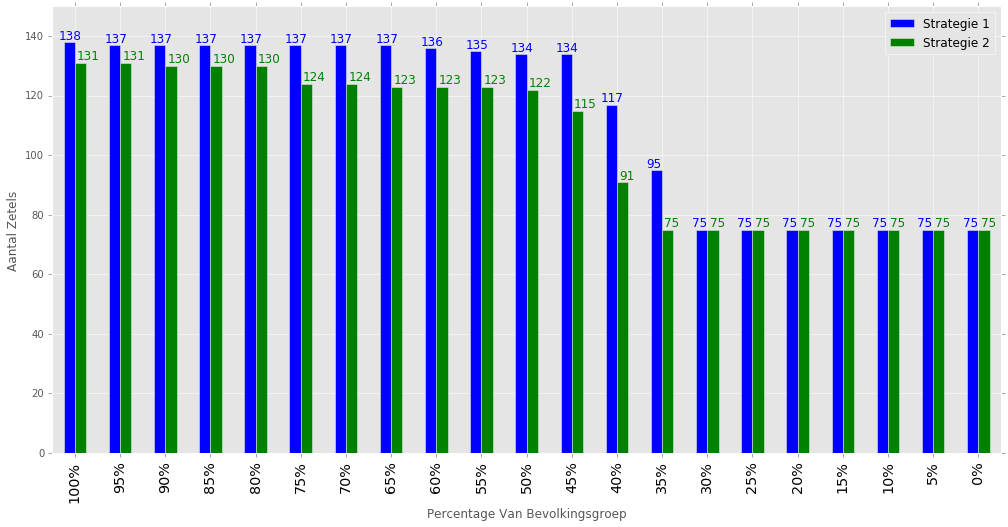
\includegraphics[width=\linewidth]{percentages_van_provincialenS1S2.png}

			\caption{Grafiek met overzicht van het maximum aantal zetels wat behaald kon worden wanneer een bepaald percentage van de provinciale kiezers zich committeerde aan strategie 1 of strategie 2.}

\label{fig:PerP}
\end{figure}

In Figuur \ref{fig:PerP} is te zien dat wanneer slechts 45\% van de provinciale kiezers zich had gecommitteerd aan strategie 1, er maar vier provinciale kandidaten afgevallen zouden zijn. Bij 35\% van de provinciale kiezers zouden er nog twintig meer provincialen in de Tweede Kamer plaats zouden hebben genomen daadwerkelijk bij de offci\"{e}le verkiezingsuitslag al het geval was (75 provincialen in de Tweede Kamer na offci\"{e}le einduitslag). Voor strategie 2 is te zien dat bij slechts 50\% van de provinciale kiezers er nog altijd veertig provincialen meer in de Tweede Kamer plaats zouden hebben genomen dan daadwerkelijk bij de offci\"{e}le einduitslag het geval was.


 




\paragraph{Tegenstrategie.}
Vanuit de literatuur is er geen directe indicatie te vinden die erop wijst dat er daadwerkelijke anti-provinciale sentimenten bestaan bij Randstedelingen. De literatuur beschrijft wel een gebrek aan een Randstad-identiteit bij inwoners van de Randstad \citep{meijers2001deltametropool,terlouw2010randstad}. Volgens \cite{terlouw2010randstad} echter is het goed mogelijk dat er wel een Randstedelijke identiteit kan ontstaat wanneer er besloten wordt om één grote Randstad-provincie te gaan vormen. Hoewel het vanuit het huidige tijdsbeeld onwaarschijnlijk lijkt dat de Randstedelingen gezamenlijk een (tegen)strategie zullen uitvoeren om te voorkomen dat de provincialen in hogere mate vertegenwoordigd zullen worden in de Tweede Kamer, is het niet onmogelijk dat de Randstedelingen (of een andere groep zoals bijvoorbeeld een groep bestaande uit Randstedelingen én provincialen) op termijn een (tegen)strategie zullen uitvoeren. 


